%\section{DEFINITION AND DCC INSERTION FLOW}
\section{FRAMEWORK}
\label{sec:DEF}
\begin{figure}
	\centering
	\includegraphics[width=0.9\columnwidth]{flow.png}
	\caption{DCC insertion flow}
	\label{fig:flow}
\end{figure}
\begin{comment}
\begin{figure}
	\centering
	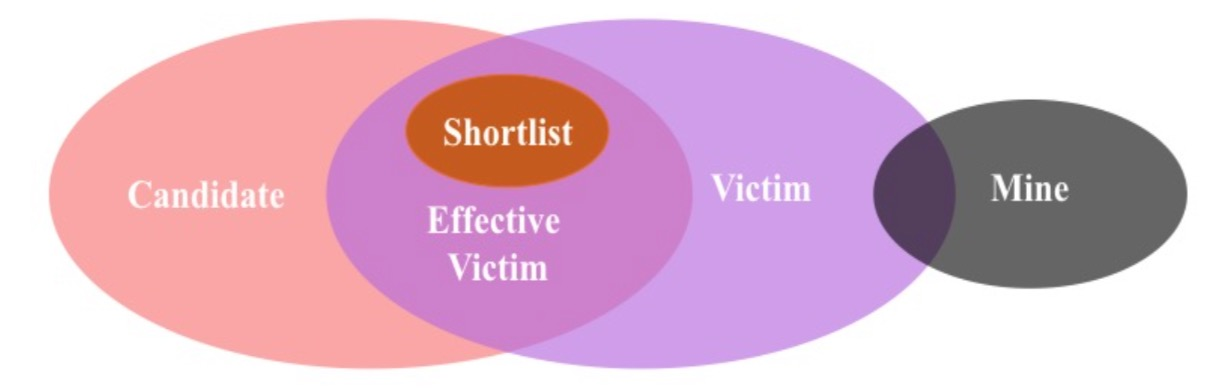
\includegraphics[width=0.9\columnwidth]{pathset.png}
	\caption{Classification of critical paths}
	\label{fig:set}
\end{figure}
\end{comment}
The overall flow of the proposed framework for DCC insertion/deployment is depicted in Figure~\ref{fig:flow}. The proposed framework focuses on the two issues: 
\begin{enumerate}
	\item \textbf{Overhead minimization}: Attacking all critical paths may be infeasible or may increase the used DCC count, which denotes the area overhead of the attack. Thus, the framework must filter/classify critical paths to make the attack successful and to minimize the DCC count. 
	\item \textbf{Workload variations}: Because users' workload highly impact the degradation of logic paths, the proposed framework must consider users' countless operational modes (i.e., workload). To be workload-aware, the problem of selecting target paths to be attacked is transform to a graph problem, which can be solved using the existing algorithms. 
\end{enumerate}


The section is organized as follows: Section~\ref{sec:DEF:CP} discusses the classification of critical paths, Section~\ref{sec:shortlist} details the workload-aware methodology to select target paths to be attacked, and Section~\ref{sec:SAT} introduces the SAT-based formulation of DCC insertion/deployment.
\subsection{Classification of Critical Paths}
\label{sec:DEF:CP}
Given a critical path, the path is classified into three groups: \textit{Shortlist}, \textit{Candidate}, and \textit{Mine}, depending on the lifetime\footnote{The lifetime of a critical path is defined as when the timing violation occurs on the path, in the presence of aging.} distribution\footnote{Given a critical path, a DCC deployment on the associated clock paths results in an individual lifetime value of the critical path. Thus, numerous DCC deployments on the associated clock paths forms the lifetime distribution of the path.} of the critical path, under all possible DCC deployments on the associated clock network. The lifetime distribution of the path is further analyzed with three lifetime intervals, which are defined as follows: $[0, n - \varepsilon]$, $[n - \varepsilon, n + \varepsilon]$, and $[n + \varepsilon, \infty]$, where $n$ is the expected circuit lifetime under the proposed HTH attack and $\varepsilon$ is mximum tolerable error. The lifetime distributions of the path in the three intervals determine the classification of the critical path. 
\begin{itemize}
	\item \textit{Candidate}: A critical path is defined as a candidate if there at least exists one DCC deployment, which leads the critical path to fail within $[n - \varepsilon, n + \varepsilon]$\footnote{Because of the effects of PVs and workload variations, it is impossible to precisely control the circuit lifetime at the expected lifetime $n$, thus, the Trojan attack, controlling the circuit lifetime within $[n - \varepsilon, n + \varepsilon]$ is accepted/desired. Therefore, the lifetime interval $[n - \varepsilon, n + \varepsilon]$ is defined as \textit{desired lifetime interval}.}.
	\item \textit{Mine}: A critical path is defined as a mine if it satisfies the following conditions: ($i$) The path is not a candidate. That is, on the associated clock paths of the critical path, there is no DCC deployment to control the path lifetime within $[n - \varepsilon, n + \varepsilon]$. ($ii$) On the associated clock paths, there at least exists one DCC deployment, which leads the critical path to fail within $[0, n - \varepsilon]$, i.e., it lead the critical path to fail prematurely.
	\item \textit{Shortlist}:  Critical paths in \textit{shortlist} is the subset of \textit{Candidate}, which are selected as target paths to be attacked. Attacking such paths involves deploying DCCs on their associated clock paths.
\end{itemize}

To be PV-aware, while classifying critical paths, we conduct Monte-Carlo simulation on the delay of logic path in a statistical manner. The simulation is performed by imposing extra V\textsubscript{th} offset (i.e., $\Delta V_{th\_pv}$ ) on each transistor of logic path. Then, we check the setup-time constraint using Equation~(\ref{eq:setup}), considering the correlation of PVs and BTI, which is introduced in the next subsection. 

\subsection{Path Delay Estimation considering the Correlation between PVs and BTI}
In this subsection, we discuss the correlation between PVs and BTI. The correlation is a long-term phenomenon that bridge the V\textsubscript{th} differences among the transistors over a period. Further, a positive/negative V\textsubscript{th} offset leads to a higher/lower fresh V\textsubscript{th}, causing a lower/higher aging speed. Therefore, the gap between high and low V\textsubscript{th} will be gradually converged, letting threshold voltages of transistors, whose fresh ones are different, reach a convergent value. We use a model proposed in~\cite{gomez2016early} to estimate the correlation between fresh V\textsubscript{th} offset and BTI effects:
\begin{equation}
	\centering
	\fontsize{9}{9} \selectfont
	\Delta V_{th\_bti} = (1 - S_{v} \cdot \Delta V_{th\_pv})  \cdot A \cdot \alpha^n \cdot t^n
	\label{eq:cor}
\end{equation}
where $\Delta V_{th\_pv}$ is the fresh V\textsubscript{th} offset due to PV. $\Delta V_{th\_bti}$ is the BTI-induced V\textsubscript{th} shift, $\alpha$ is the stress duty cycle, $A$ is $3.9 \times 10^{-3} V \cdot s^{-1/_5}$, $n$ is time exponential constant, 0.2 for used technology, and $S_{v}$ is a constant which can be extracted by fitting HSPICE simulation results in 45nm TSMC technology. 

%------- Shortlist selection --------------------------------------------------------------------------------------------------
\subsection{Selection of Target Paths (Shortlist) to be attacked}
\label{sec:shortlist}
\begin{figure}
	\centering
	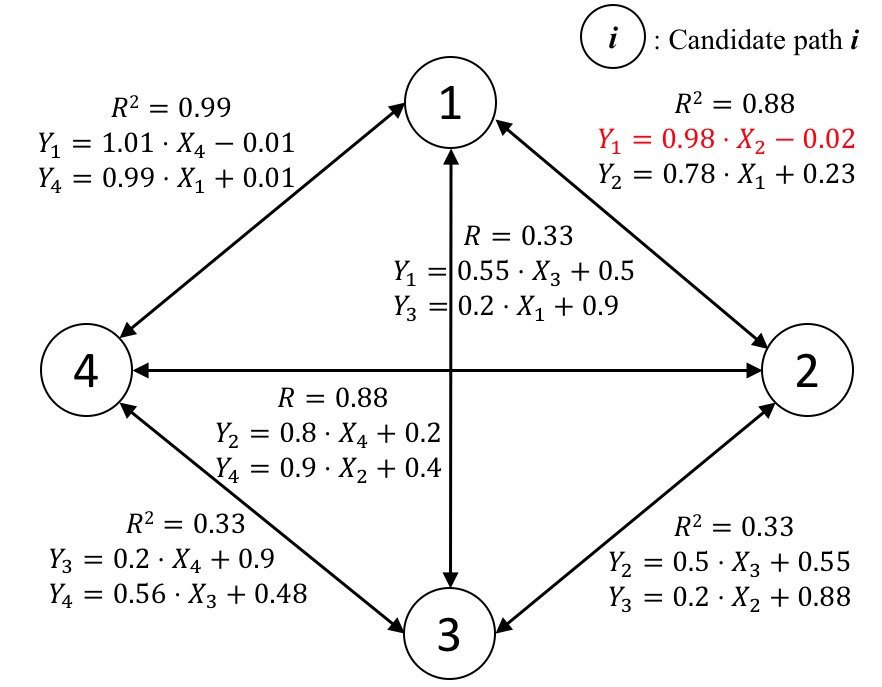
\includegraphics[width=0.9\columnwidth]{graph.png}
	\caption{Example of graph used in choosing targets}
	\label{fig:graph}
\end{figure}

%If an attacked critical path always ages as estimated (i.e., under worst-case aging), a successful attack can be obtained just by inserting DCCs on its associated clock paths. However, uncertainty of user-dependent operational modes (e.g., watching video, playing games) can influence/vary the aging behavior. Therefore, we must ensure that the attack will succeed under any operational mode. We make the following assumption, which is also used in Section~\ref{sec:lt_estimation} to estimate the lifetime of attacked designs:
The uncertainty of user-dependent operational modes (e.g., watching video, playing games) can influence/vary the aging behavior of logic paths. Therefore, we must ensure that the attack will succeed under any operational mode. We make the following assumption, which is also used in Section~\ref{sec:lt_estimation} to estimate the lifetime of attacked designs:

\textit{"Every operational mode causes at least one candidate path to undergo worst-case aging."}

In other words, no matter how users operate the design, at least one candidate path in the design undergoes worst-case aging. Moreover, an operational mode, which causes one path to undergo worst-case aging, is defined as the \textit{critical operational mode} of the path. This way, the union of critical operational modes of all candidate paths is equivalent to the universe of operational modes. Therefore, attacking all candidate paths is a na�ve method to guarantee the successful attack, based on the assumption. Nevertheless, it is very costly and may be impossible.

Therefore, after observing the relationship among aging of paths, we find that the aging behaviors of many paths are highly correlated. If several paths are highly correlated in terms of aging behavior, one operational mode can lead all of them to age to a similar extent. Thus, we can simply attack one out of those highly correlated paths to cover multiple operational modes. For example, given two critical paths $A$ and $B$. Their critical operational modes are $O_{A}$ and $O_{B}$, respectively. Assume that $A$ and $B$ are highly correlated in terms of aging behavior. Because $A$ and $B$ age similarly/closely, $O_{A}$ causes $A$ to age in the worst-case and also causes $B$ to age severely. Consequently, even if we simply attack path $A$, not only $O_{A}$ but also $O_{B}$ can make the attack successful (i.e., shorten the lifetime of path $A$ to the interval [$n - \varepsilon, n + \varepsilon$]). This property helps reduce the count of targeted paths to be considered/formulated.
To choose the attack targets (shortlist), we transform the relationship of paths to a directed graph (also known as digraph). In Figure~\ref{fig:graph}, vertices represent candidates and arcs (i.e., directed edges) are correlation coefficients ($R^2$) and linear regression equations between each pair of vertices. Each arc has a regression equation, whose coefficients are obtained by running functional simulation. $X_{i}$ denotes the worst-case aging rate of path $i$, whose exact value will be introduced in Section [Undefined]. $Y_{j}$ denotes the aging rate of path $j$ predicted based on the linear regression equation. Consider the orange equation in Figure~\ref{fig:graph}:

\begin{equation}
	\centering
	\fontsize{8}{8} \selectfont
	Y_{1} = 0.98 \cdot X_{2} - 0.02
\end{equation}

Given the worst-case aging rate of vertex/path 2, $X_{2}$, the aging rate of vertex/path 1, $Y_{1}$, can be predicted as 0.98 multiplied by $X_{2}$ minus 0.02.
Before the shortlist is determined by selecting a subset of candidates in the graph, we can simplify the graph by removing some arcs which indicate the relationships of weak aging correlation between pairs of paths.

The cost of our proposed HTHs is the inserted DCC count. To minimize the cost, we select minimum-sized targets to cover all candidate paths, that is, to dominate all candidate paths in the digraph, such that all users' operational modes are considered in the proposed Trojan attack, based on the assumption. This problem is similar to a classical digraph problem, \textbf{Minimum Dominating Set (MDS)}:

\textit{On digraph $G = (V, E)$, find a minimum-sized set of vertices $S \subseteq V$ such that $\forall y \notin S$, $\exists x \in S$, there exists an arc from $x$ to $y$. And we say that $y$ is dominated by $x$}.

Therefore, the problem of selecting target paths to be attacked is transformed to a MDS-related digraph problem, which can be solved using the existing algorithms proposed in \cite{ore1962theory}\cite{natarajan1978optimum}.
%------- SAT  --------------------------------------------------------------------------------------------------


\subsection{SAT-based Problem Formulation and Encoding for DCC Deployment}
\label{sec:SAT}
\begin{comment}
	\begin{figure*}[!ht]
    	\centering
    	\subfigure[A DCC deployment leads path $p$ to fail prematurely]{
    		\label{fig:sub:upper}
        		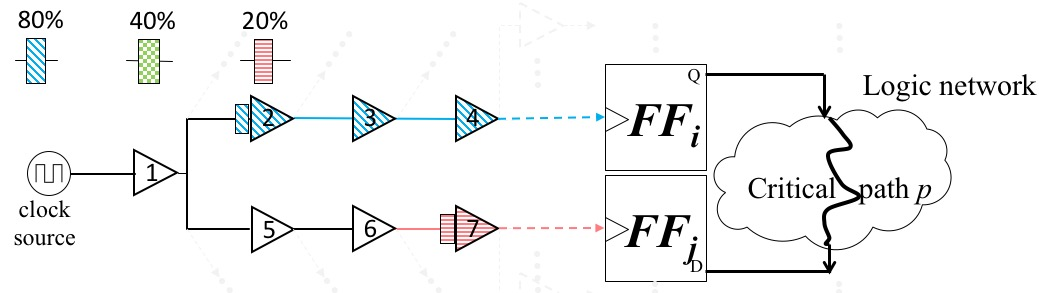
\includegraphics[width=0.9\columnwidth]{upper.png}
    	}
   	\hspace{0.1cm}
    	\subfigure[A DCC deployment leads path $p$ to fail post-maturely]{
    		\label{fig:sub:lower}
        		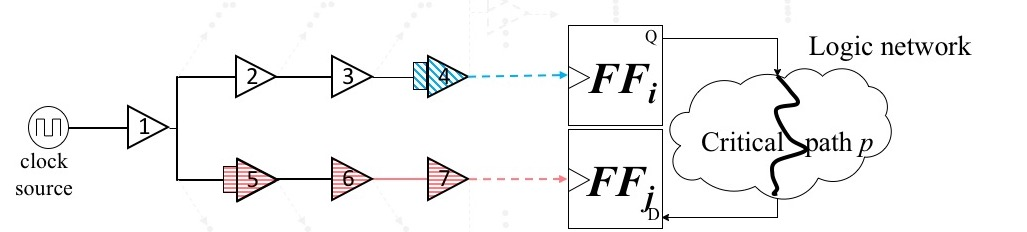
\includegraphics[width=0.92\columnwidth]{lower.png}
    	}
    	\caption{Illustrative example for the proposed framework based on DCC deployment/insertion}
    	\label{fig:en}
	\end{figure*}
\end{comment}
\begin{figure}
    	\centering
        	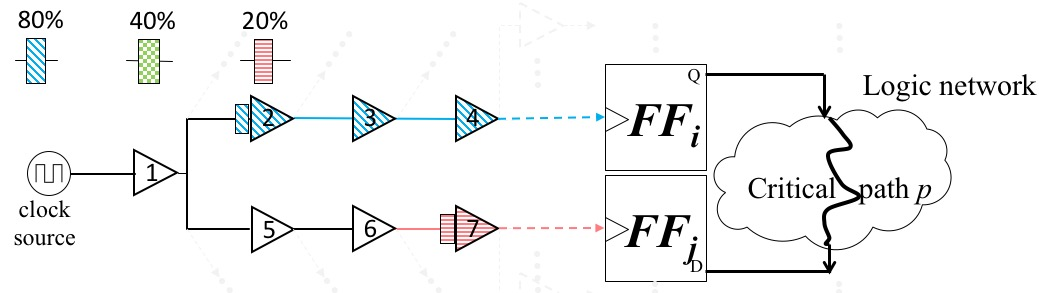
\includegraphics[width=0.9\columnwidth]{upper.png}
       	\caption{A DCC deployment leads path $p$ to fail prematurely}
    	\label{fig:sec:prefail}
\end{figure}
After the shortlist (i.e., target paths to be attacked) is determined, the problem of DCC deployment on their associated clock paths is formulated as a \textbf{Boolean satisfiability (SAT)} problem. The key of the framework is to represent the problem in \textit{conjunctive normal form} (CNF). A CNF representation is a conjunction of one or more clauses, where each clause is a disjunction of one or more Boolean variables. Thus, DCC deployment/insertion needs to be encoded into Boolean representation before being transformed into a SAT-based formulation. Assume that a total of 3 types of DCCs can be chosen (i.e., 20\%, 40\%, and 80\% DCCs). Including the DCC-free case where no DCC is inserted, there are 4 possibilities of DCC insertion for each clock buffer. Given a clock buffer $p$, the four possibilities of DCC insertion at the input of buffer $p$ can be encoded as follows using two Boolean variables $B_{p,2}$ and $B_{p,1}$:

{\small
\begin{tabular}{ c c c }
   & DCC type & $\left\{B_{p,2},B_{p,1}\right\}$ \\
  (1)\quad & None & \{0,0\} \\
  (2)\quad & 20\% &  \{0,1\} \\
  (3)\quad & 40\% &  \{1,0\} \\
  (4)\quad & 80\% &  \{1,1\} \\
\end{tabular}}

To control the circuit lifetime within $[n - \varepsilon, n + \varepsilon]$, timing constraints of DCC deployments are formulated in the SAT-based problem. The formulations of timing constraints depend on the classification of critical paths.
\begin{enumerate}
	\item Paths in the shortlist (i.e., targets): The lifetime (i.e., when timing violations occur) of shortlist paths dominate the lifetime of attacked designs. To control the lifetime of shortlist paths within $[n - \varepsilon, n + \varepsilon]$, on their associated clock paths, we formulate all DCC deployments, which lead the path to fail prematurely or post-maturely (i.e., within $[ 0, n - \varepsilon]$ or within $[ n + \varepsilon, \infty]$), such that the SAT solver does not output the corresponding deployment in the result if the CNF is satisfiable.
	\item Other paths (paths not in the shortlist): While attacking shortlist paths, the DCC deployment, on the clock paths of shortlist paths, may cause the premature failure of other paths not in shortlist, due to the common clock network, making the proposed Trojan attack premature and inaccurate. Thus, on the associated clock paths of other paths not in shortlist, we formulate all DCC deployments,  which lead the paths to fail prematurely (i.e., within $[ 0, n - \varepsilon]$), such that the SAT solver does not output the corresponding deployment in the result if the CNF is satisfiable.
\end{enumerate}

Consider the example in Figure~\ref{fig:sec:prefail}, where the 80\% and 20\% DCCs are inserted at the inputs of buffer 2 and 7, respectively. Assume that the critical path $p$ is in shortlist. If the DCC deployment will lead the path $p$ to fail prematurely (i.e., path fail within $[ 0, n - \varepsilon]$), then the following clause
\begin{gather*}
	\fontsize{9}{7} \selectfont
	\mbox{($A_{1} \lor A_{0} \lor \neg B_{1} \lor B_{0} \lor C_{1} \lor C_{0}$) } 
\end{gather*}
will be generated and added into CNF, such that the solver will not output the corresponding DCC deployment in the result if the CNF is satisfiable.

\begin{comment}
Consider the other example in Figure~\ref{fig:sub:lower}, where the 80\% and 20\% DCCs are inserted at the inputs of buffer 4 and 5, respectively. Assume again that the critical path $p$ is in shortlist. If the DCC deployment will lead the path $p$ to fail post-maturely (i.e., path fail within $[ n + \varepsilon, \infty]$), then the following clause
\begin{gather*}
	\fontsize{9}{7} \selectfont
	\mbox{($A_{1} \lor A_{0} \lor B_{1} \lor B_{0} \lor C_{1} \lor \neg C_{0}$) } 
\end{gather*}
will be generated and added into CNF, such that the solver will not output the corresponding DCC deployment in the result if the CNF is satisfiable.
\end{comment}
For SAT-based formulation, our proposed problem of DCC deployment is transformed into CNF clauses. The CNF clauses are solved by SAT solver such as MiniSat and we can find the locations and types of inserted DCCs by decoding the output from the solver.



